
\section{Analysis optimisation}
\label{sec:optimisation}

One motivation for this work was to quantify which aspects
of the performance of the LHC detectors need to be improved
the most in order to maximise the significance of the observation
of double Higgs production in the $4b$ final state.
%
In this section we explore how the post-MVA
results with the baseline settings,
summarized in the previous section, are modified when some of
these settings are modified.
%
In particular we will explore the dependence of the results on
the $b$-tagging probability $f_b$, the light jet mistag rate
$f_l$, as well on the four-momentum smearing fraction $\sigma_E$,
see Eq.~(\ref{eq:smearing}).
%
The variations of the analysis
settings that we will explore are collected in
Table~\ref{sec:variations}.

%%%%%%%%%%%%%%%%%%%
\begin{table}[h]
  \centering
  \begin{tabular}{|c|c|c|c|}
\hline
    Scenario  &  $f_b$  &  $f_l$  &  $\sigma_E$ \\
    \hline
    \hline
    Baseline  &  0.8   &   0.01  &  5\% \\
    \hline
    A        &  0.9   &   0.01  &  5\% \\
    B        &  0.7   &   0.01  &  5\% \\
    C        &  0.8   &   0.005  &  5\% \\
    D        &  0.8   &   0.02  &  5\% \\
    E        &  0.9   &   0.005  &  3\% \\
    F        &  0.9   &   0.005  &  7\% \\   
    \hline
  \end{tabular}
  \caption{\small The baseline settings for the $b$-jet
    tagging probability, the light jet mistag rate $f_l$
    and the momentum resolution $\sigma_E$, compared
    to the various scenarios that we discussed in this section.
\label{sec:variations}
  }
  \end{table}
%%%%%%%%%%%%%%%%%%%


Given that we have found in the previous section that the
category with highest discrimination power is the boosted one,
in this section we concentrate on it,
by comparing our baseline results from Table~\ref{table:cutflowMVA}
with the new scenarios.
%
Each time of the parameters in Table~\ref{sec:variations}
 has been changed, the MVA has been retrained to optimise the
new information contained in the various scenarios.
%
This is important since for example, when we vary $f_b$
or $f_l$, the relative composition of the multijet
background will change, and this can translate into
modifications of the kinematical variables used for
the MVA training.
%
Similarly, if the momentum resolution is modified,
the weight of the different variables in the MVA
will be altered, in particular the invariant mass
of Higgs candidates $m_h$.


The results of this optimisation study are collected in
Table~\ref{table:cutflowMVAoptimisation}.
%
There we compare the results for the number of signal
and background events $N_{\rm ev}$ expected at the
HL-LHC, the signal significance, and the $S/B$ ratio,
for our nominal settings and for the variations
of the analysis settings.

%%%%%%%%%%%%%%%%%%%%%%%%%%%%%%%%%%%%%%%%%%%%%%%%%%%%%
\begin{table}[t]
  \centering
  \begin{tabular}{c||c|c|c|c}
    \hline
    \multicolumn{5}{c}{Boosted category}\\
    \hline
    \hline
 Scenario &    \multicolumn{2}{c|}{$N_{\rm ev}$} &  $S/\sqrt{B}$  & $S/B$ \\
       &   Signal & Back   &     &    \\
 \hline
 \hline
   Baseline   & 107 & 1040 & 3.31  & 0.10\\
   \hline
   &  &   &   &   \\
   &  &   &   &   \\
   &  &   &   &   \\
   &  &   &   &   \\
         &  &   &   &   \\
   \hline
  \end{tabular}
  \caption{\small
Number of signal
and background events $N_{\rm ev}$ expected at the
HL-LHC, signal significance and $S/B$ ratio
for the nominal settings and for the variations
of the analysis settings, summarized
in  Table~\ref{sec:variations}.
 \label{table:cutflowMVAoptimisation}
  }
\end{table}
%%%%%%%%%%%%%%%%%%%%%%%%%%%%%%%%%%%%%%%%%%%%%%%%%%%%%

Neglecting the
contribution from light jet fakes,
it is easy to estimate how $S/\sqrt{B}$ should
scale with $f_b$: since we have two double-$b$-tagged jets
both in signal and background events, one should find that
\be
\lp \frac{S}{\sqrt{B}} \rp _{f_b}\Bigg/
\lp \frac{S}{\sqrt{B}} \rp_{f_b'}
\simeq \frac{f_b^2}{f_b'^2} \, .
\ee
By comparing this expectations with the numbers of
Table~\ref{table:cutflowMVAoptimisation}, we see that there
is a reasonable agreement in the boosted category,
as expected since it is dominated by the irreducible
$4b$ component of the QCD multijet background.

The most aggressive scenario is the one in which the $b$-tagging
is improved up an efficiency $f_b=0.9$, while at the same
time the light jet fake rate is reduced down to $0.5\%$, while
at the same time the momentum resolution has been decreased
to $\sigma_E=3\%$.
%
In this scenario, the signal significance of the boosted category
increases to AAA, to be compared to BBB with the baseline settings.





  \subsection{The role of the overlap between different categories}
\label{sec:overlap}

As has been discussed in Sect.~\ref{sec:analysis}, while the optimization of each
category is performed in an inclusive analysis, after having determined the order
of significance of the separate categories. we turn to a exclusive analysis,
in order that
we can combine consistently the results from the various topologies without double
counting.
%
Here we discuss the role of the overlap
between  different categories, which is of course ignored in the final exclusive
analyses.
%
The idea is to understand how significant the information is on which events satisfy the requirements
of more than one category at the same time.

To illustrate the role of the overlap between the different categories, in
Fig.~\ref{fig:categorisationHisto} we show the fraction of events that satisfy the requirements
of one or more categories, for signal and background events.
%
We consider the following cases:
\begin{itemize}
\item events that satisfy the requirements of one category (resolved,
  intermediate or boosted),
\item events that satisfy the conditions of both the resolved and the intermediate categories,
\item and the same for events that fall both
  into the resolved and boosted categories.
\end{itemize}
 Note that by construction, there is no overlap between the boosted
  and intermediate categories due to the
 orthogonal jet multiplicity cuts.

%%%%%%%%%%%%%%%%%%%%%%%%%%%%
\begin{figure}[t]
\begin{center}
%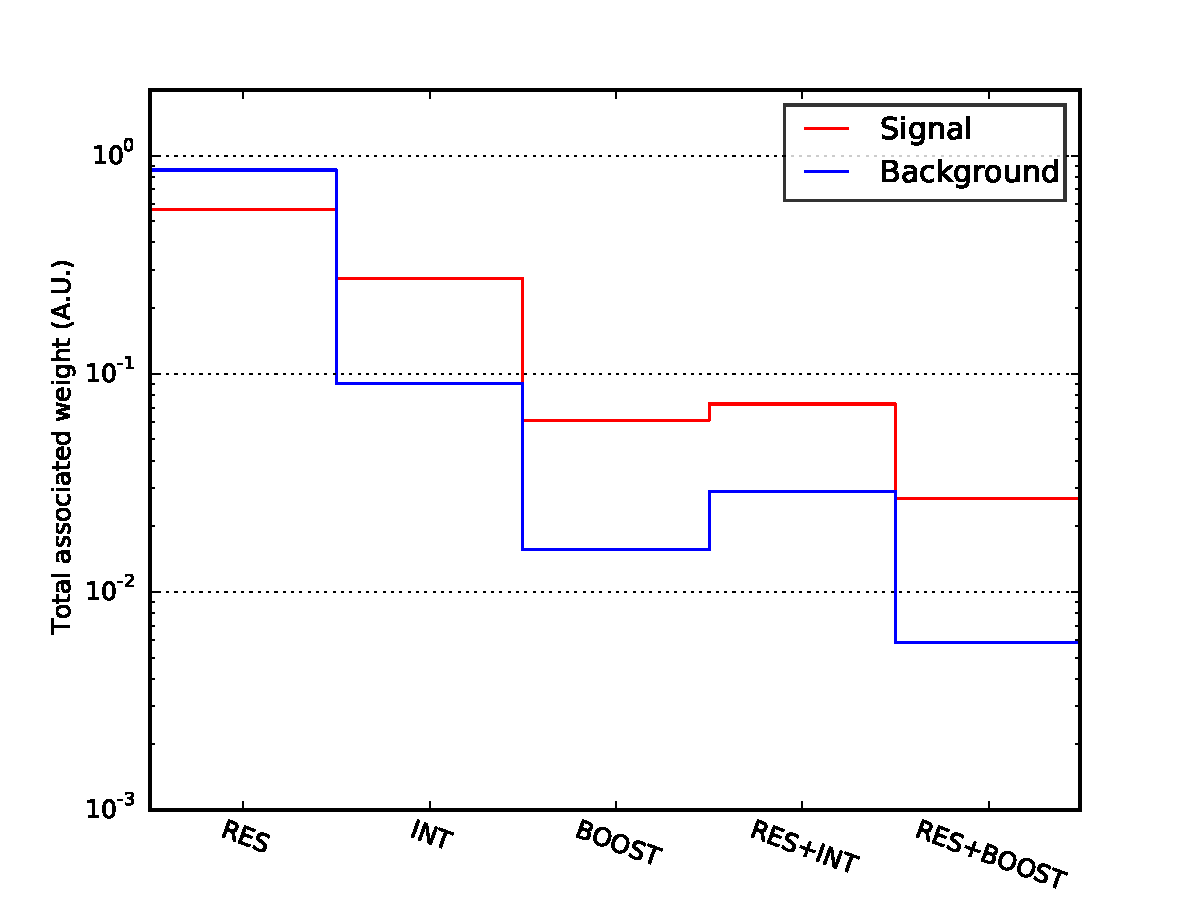
\includegraphics[width=0.65\textwidth]{plots/overlap_categories_C1.pdf}
\caption{\small The fraction of events that satisfy the requirements
  of one or more categories, for signal and background events.
  %
  By construction, there is no overlap between the boosted
  and intermediate categories due to the
   orthogonal jet multiplicity cuts. {\bf update including event weights}
}
\label{fig:categorisationHisto}
\end{center}
\end{figure}
%%%%%%%%%%%%%%%%%%%%%%%

As we can see from Fig.~\ref{fig:categorisationHisto}, an large majority of the events
belong to the resolved category, specially in the background case ($\sim 90\%$) but
also a large part of the signal ($\sim 60\%$).
%
In all the other categories, including
the overlaps, signal events are more likely to belong to them than
background events.
%
In the intermediate category, we have around $\sim$30\% of the signal
events and $\sim$10\% of the background events.
%
For the boosted case, we find $\sim$ 6\% of signal events and
$\sim$2\% of background events.
%
We also find that the overlap between the boosted and the other categories
is small: none with the intermediate (by construction), and then $\sim$3\%
($\sim$0.05\%) of the signal (background) events.
%
The overlap between the resolved and the intermediate is also smaller
than the two categories separately: $\sim$7\%
($\sim$ 3\%) for signal (background) events.

Therefore, from the results of Fig.~\ref{fig:categorisationHisto}
we can conclude that the effect of the overlap between categories would
be small correction with respect to the exclusive selection approach
that we use in this work.
%
Note also that while the majority of signal events are in the resolved
category, since the fraction of background events is also larger,
it is advantageous to use the small fraction of events in the boosted category
since the suppression of the background in this category is larger
than in the others.
